%!TEX program = xelatex
%!TEX root = Algebra_1.tex
%%Usar makeindex -s indexstyle.ist arquivo.idx no terminal para gerar o {\'\i}ndice remissivo agrupado por inicial
%%Ap\'os executar pdflatex arquivo
\chapter{Conceitos B\'asicos} % (fold)
\label{cha:conceitos_basicos}

\begin{definicao}
	Uma \textbf{proposi\c{c}\~ao} \'e todo conjunto de palavras ou s{\'\i}mbolos ao qual podemos atribuir um \textbf{valor l\'ogico}.
\end{definicao}

\begin{definicao}
	Diz-se que o \textbf{valor l\'ogico} de uma proposi\c{c}\~ao \'e ``verdade'' (V) se a proposi\c{c}\~ao \'e verdadeira ou ``falsidade'' (F) se a proposi\c{c}\~ao \'e falsa.
\end{definicao}

\begin{exemplos}
	Julgue se as seguintes senten\c{c}as s\~ao ou n\~ao proposi\c{c}\~oes:
	\begin{enumerate}[label={\arabic*})]
		\item Todo n\'umero primo \'e {\'\i}mpar.
		\begin{solucao}
			Essa seten\c{c}a \'e uma proposi\c{c}\~ao de valor l\'ogico "Falsidade."
		\end{solucao}

		\item $x^2 + y^2 \ge 0$ para todos $x$, $y \in \real$.
		\begin{solucao}
			Esse seten\c{c}a \'e uma proposi\c{c}\~ao de valor l\'ogico "Verdade".
		\end{solucao}

		\item Amanh\~a ir\'a chover.
		\begin{solucao}
			Essa senten\c{c}a n\~ao \'e uma proposi\c{c}\~ao. N\~ao \'e poss{\'\i}vel atribuir um valor l\'ogico a ela.
		\end{solucao}
	\end{enumerate}

\end{exemplos}

\section{Princ{\'\i}pio da n\~ao contradi\c{c}\~ao e do terceiro exclu{\'\i}do} % (fold)
\label{sec:principio_da_nao_contradicao_e_do_3}
\begin{enumerate}[label={\roman*})]
	\item Uma proposi\c{c}\~ao n\~ao pode ser verdadeira e falsa ao mesmo tempo.
	\item Toda proposi\c{c}\~ao ou \'e verdadeira ou \'e falsa, isto \'e, verifica-se sempre um destes casos e nunca um terceiro.
\end{enumerate}

Assim esses princ{\'\i}pios afirmam que:
\begin{center}
	``Toda proposi\c{c}\~ao tem um, e um s\'o, dos valores l\'ogicos \textbf{verdade} ou \textbf{falsidade}.''
\end{center}

De modo geral vamos trabalhar com proposi\c{c}\~oes da forma:
\begin{enumerate}[label={\roman*})]
	\item Se $\mathbb{H}$, ent\~ao $\mathbb{T}$.

	Aqui $\mathbb{H}$ \'e chamado de hip\'otese e $\mathbb{T}$ de tese. Neste tipo de proposi\c{c}\~ao iremos admitir que $\mathbb{H}$ \'e uma verdade e precisaremos provar que $\mathbb{T}$ \'e verdade. Ou seja precisamos construir um argumento que justifique $\mathbb{T}$ ser verdadeira \`a partir do fato de $\mathbb{H}$ ser verdadeira.

	\item $\mathbb{H}$ se, e somente se, $\mathbb{T}$ ou $\mathbb{H}$ se, e s\'o se, $\mathbb{T}$.

	Esse tipo de proposi\c{c}\~ao ser\'a decomposta em duas proposi\c{c}\~oes no formato anterior. Isto \'e:
	\begin{enumerate}[label={\alph*})]
		\item Se $\mathbb{H}$, ent\~ao $\mathbb{T}$.
		\item Se $\mathbb{T}$, ent\~ao $\mathbb{H}$.
	\end{enumerate}

	No primeiro caso admitimos $\mathbb{H}$ verdadeira e provamos que $\mathbb{T}$ tamb\'em \'e verdadeira e no segundo caso admitimos que $\mathbb{T}$ \'e verdadeira e provamos que $\mathbb{H}$ \'e verdadeira.
\end{enumerate}

Para demonstrarmos uma proposi\c{c}\~ao precisamos deduz{\'\i}-la de proposi\c{c}\~oes previamente comprovadas como verdadeiras. Assim uma demonstra\c{c}\~ao \'e a determina\c{c}\~ao de uma verdade e \'e constru{\'\i}da atrav\'es de uma sequ\^encia de racioc{\'\i}nios l\'ogicos, com in{\'\i}cio e fim determinados. Cada passo dessa sequ\^encia de racioc{\'\i}nio deve ter sua veracidade justificada, seja atrav\'es de outras proposi\c{c}\~oes j\'a provadas verdadeiras ou pelo uso de axiomas, que s\~ao afirma\c{c}\~oes admitidas como verdadeiras. Vamos utilizar, principalmente, tr\^es formas de demonstrar uma proposi\c{c}\~ao, a saber:
\begin{enumerate}[label={\roman*})]
	\item Demonstra\c{c}\~ao direta;
	\item Demonstra\c{c}\~ao por contraposi\c{c}\~ao;
	\item Demonstra\c{c}\~ao por contradi\c{c}\~ao ou redu\c{c}\~ao ao absurdo.
\end{enumerate}

Assim numa proposi\c{c}\~ao do tipo:
\begin{center}
	Se $\mathbb{H}$, ent\~ao $\mathbb{T}$.
\end{center}

Para demonstr\'a-la de forma \textbf{direta} devemos admitir a hip\'otese $\mathbb{H}$ verdadeira, e utilizando de uma sequ\^encia de passos cuja veracidade podemos comprovar, chegar \`a conclus\~ao que a tese $\mathbb{T}$ tamb\'em \'e verdadeira.

Na \textbf{demonstra\c{c}\~ao por contraposi\c{c}\~ao}, iremos supor que a $\mathbb{T}$ \'e \textbf{falsa} e novamente atrav\'es de uma sequ\^encia de passos que podemos justificar como verdadeiros, devemos chegar \`a conclus\~ao que a hip\'otese $\mathbb{H}$ tamb\'em \'e falsa. Se conseguirmos chegar a essa conclus\~ao ent\~ao a proposi\c{c}\~ao original ser\'a verdadeira.

Por \'ultimo, na \textbf{demonstra\c{c}\~ao pro contradi\c{c}\~ao} ou \textbf{redu\c{c}\~ao ao absurdo}, iremos admitir que a hip\'otese $\mathbb{H}$ \'e verdadeira e que a tese $\mathbb{T}$ \'e falsa. Usando essas suposi\c{c}\~oes devemos chegar \`a alguma conclus\~ao contradit\'oria, isto \'e, precisamos obter alguma informa\c{c}\~ao que seja verdadeira e falsa ao mesmo tempo. Nesse caso, significa que nossa tese $\mathbb{T}$ deve ser obrigatoriamente verdadeira, e com isso a proposi\c{c}\~ao tamb\'em ser\'a verdadeira.

% section pr{\'\i}ncipio_da_n\~ao_contradi\c{c}\~ao_e_do_3 (end)

% chapter conceitos_b\'asicos (end)

\chapter{No{\c c}{\~o}es de Teoria de Conjuntos}
\section{Conceitos b{\'a}sicos}

Um conjunto {\'e} uma ``cole{\c c}{\~a}o'' ou ``fam{\'\i}lia'' de elementos.

Usaremos letras mai{\'u}sculas do alfabeto para denotar os conjuntos e denotaremos elementos de um dado conjunto por letras min{\'u}sculas do alfabeto.

Dado um conjunto $A$, para indicar o fato de que $x$ {\'e} um elemento de $A$, escrevemos:
\[
	x \in A.
\]

Para dizer que um elemento $x$ n{\~a}o pertence ao conjunto $A$, escrevemos:
\[
	x \notin A.
\]

Um conjunto sem elementos {\'e} chamado de \textbf{conjunto vazio}. Tal conjunto {\'e} denotado por $\emptyset$ ou por $\{\ \}$.

Dado um conjunto $A$ e $x$ um elemento, ocorre sempre uma das seguintes situa\c{c}\~oes:
\[
	x \in A \mbox{ ou } x \notin A.
\]

Al{\'e}m disso, para dois elementos $x$, $y \in A$, ocorre exatamente uma das seguinte situa\c{c}\~oes:
\[
	x = y \mbox{ ou } x \neq y.
\]

\section{Descri{\c c}{\~a}o de um conjunto}

Um conjunto $A$ pode ser dado pela simples listagem dos seus elementos, como por exemplo:
\begin{align*}
	A &= \{1,2,3,4,5\}\\
	B &= \{verdade, falso\}.
\end{align*}

Um conjunto tamb{\'e}m pode ser dado pela descri{\c c}{\~a}o das propriedades dos seus elementos, como por exemplo:
\[
	A = \{n \mid n \mbox{ \'e m{\'u}ltiplo de } 2\} = \{2,4,6,...\}.
\]

\section{Alguns conjuntos importantes}
\begin{enumerate}[label={\arabic*})]
	\item $\n = \{0,1,2,3,...\}$ o conjunto do n{\'u}meros naturais.
	\item $\n_0 = \{0,1,2,3,...\}$ o conjunto dos n{\'u}meros inteiros n{\~a}o negativos.
	\item $\z = \{...,-2,-1,0,1,2,...\}$ o conjunto dos n{\'u}meros inteiros.
	\item $\rac = \left\{\dfrac{p}{q} \mid p,q \in \z, q \neq 0 \right\}$ o conjunto dos n{\'u}meros racionais.
	\item $\real $ o conjunto dos n{\'u}meros reais.
	\item $\real^*$ o conjunto dos n{\'u}meros reais n{\~a}o nulos.
	\item $\complex = \{a + bi \mid a,b \in \real,\ i^2 = -1\}$ o conjunto dos n\'umeros complexos.
\end{enumerate}

\begin{observacao}
	Para esses conjuntos vamos admitir como verdadeiras as propriedades b\'asicas da soma e multiplica\c{c}\~ao.
\end{observacao}
\section{Propriedades dos conjuntos}

\begin{definicao}\label{igualdade_conjuntos}
	Dados dois conjuntos $A$ e $B$, dizemos que $A$ e $B$ s{\~a}o \textbf{iguais} se, e somente se, eles t{\^e}m os mesmos elementos. Ou seja, para todo $x \in A$ também vale que $x \in B$ e para todo $y \in B$ também vale que $y \in A$. Se $A$ e $B$ s{\~a}o iguais, escrevemos $A = B$.
\end{definicao}

\begin{exemplo}
	Sejam $A = \{1,1,2,3,4,4\}$, $B = \{3,2,1,4\}$, $C = \{1,2,3\}$ e $D = \{2,3\}$. Ent\~ao de acordo com a Defini\c{c}\~ao \ref{igualdade_conjuntos} temos $A = B$ pois todo elemento de $A$ est\'a em $B$ e todo elemento de $B$ tamb\'em est\'a em $A$. Agora como $1 \in C$ e $1 \notin D$ ent\~ao $C \ne D$.
\end{exemplo}

\begin{observacao}
	Dados conjuntos $A$ e $B$, de acordo com a Defini\c{c}\~ao \ref{igualdade_conjuntos} para que $A \ne B$ basta que exista um elemento $x \in A$ de maneira que $x \notin B$ ou que exista $y \in B$ com a condição de que $y \notin A$.
\end{observacao}

\begin{definicao}\label{definicao_continencia_conjuntos}
	Se $A$ e $B$ s{\~a}o dois conjuntos, dizemos que $A$ {\'e} um \textbf{subconjunto} de $B$ ou que $A$ \textbf{est\'a contido} em $B$ ou que $B$ \textbf{cont\'em} $A$ se todo elemento de $A$ for elemento de $B$. Ou seja, se para todo elemento $x \in A$, temos $x \in B$. Nesse caso, escrevemos $A \subseteq B$ (ou $A \subset B$) ou $B \supseteq A$ (ou $B \supset A$).
\end{definicao}


Caso $A$ seja um subconjunto de $B$ mas n{\~a}o {\'e} igual a $B$, escrevemos:
\[
	A \subsetneq B.
\]

Nesse caso, dizemos que $A$ {\'e} um \textbf{subconjunto pr{\'o}prio} de $B$.

\begin{exemplos}
	Sejam $A = \{1,2,3,x,y,z\}$, $B = \{x, y\}$ e $C = \{x, y , z\}$. Temos:
	\begin{enumerate}[label={\arabic*})]
		\item $A \nsubseteq B$ pois $1 \in A$ e $1 \notin B$.
		\item $B \subsetneq A$ pois todo elemento de $B$ tamb\'em est\'a em $A$. Observe que existem elementos de $A$ que n\~ao est\~ao em $B$, por exemplo $2 \in A$ e $2 \notin B$.
		\item $B \subseteq C$ pois todo elemento de $B$ tamb\'em est\'a em $C$.
		\item $C \subseteq A$ pois todo elemento de $C$ tamb\'em est\'a em $A$.
	\end{enumerate}
\end{exemplos}

\begin{observacao}
	Dados dois conjuntos $A$ e $B$ pela Defini\c{c}\~ao \ref{definicao_continencia_conjuntos} para que $A$ \textbf{n\~ao esteja contido em} $B$ basta que exista $x \in A$ tal que $x \notin B$. Nesse caso escrevemos $A \nsubseteq B$.
\end{observacao}

Usando a defini\c{c}\~ao de contin\^encia de conjuntos, Defini\c{c}\~ao \ref{definicao_continencia_conjuntos}, podemos redefinir a igualdade de conjuntos, Defini\c{c}\~ao \ref{igualdade_conjuntos}, da seguinte forma: dados dois conjuntos $A$ e $B$
\begin{center}
	$A = B$\quad \textbf{se, e somente se,}\quad $A \subseteq B$\quad \textbf{e}\quad $B \subseteq A$.
\end{center}

Ou seja,
\begin{center}
	\textbf{se} $A = B$ \textbf{ent{\~a}o} $A \subseteq B$ \textbf{e} $B \subseteq A$.
\end{center}

Al\'em disso,
\begin{center}
	\textbf{se} $A \subseteq B$ \textbf{e} $B \subseteq A$, \textbf{ent{\~a}o} $A = B$.
\end{center}

Quando $A$ e $B$ n{\~a}o s{\~a}o iguais, escrevemos $A \neq B$. Para que $A \neq B$ devemos ter $A \nsubseteq B$ ou $B \nsubseteq A$. Isto \'e, precisamos encontrar algum elemento $x \in A$ de modo que $x \notin B$ ou ent\~ao encontrar $y \in B$ com a condição de que $y \notin A$.

\begin{proposicao}
	Dados tr\^es conjuntos $A$, $B$ e $C$ temos:
	\begin{enumerate}[label={\roman*})]
		\item $A\subseteq A$ (Reflexividade)
		\item Se $A\subseteq B \mbox{ e } B\subseteq A$, ent{\~a}o $A=B$. (Antissimetria)
		\item Se $A\subseteq B$ e $B\subseteq C$, ent{\~a}o $A\subseteq C$. (Transitividade)
	\end{enumerate}
\end{proposicao}


Considere os seguintes conjuntos:
\begin{align*}
	A &= \{ n \in \n \mid n \mbox{ {\'e} m{\'u}ltiplo de } 2\} = \{2,4,6,...\}\\
	B &= \{n \in \n \mid n \mbox{ {\'e} m{\'u}ltiplo de } 3\} = \{3,6,9,...\}.
\end{align*}


Neste caso, $2 \in A$ e $2 \notin B$, logo $A \nsubseteq B$. Por outro lado, $3 \in B$ e $3 \notin A$ e com isso $B \nsubseteq A$. Portanto, dados dois conjuntos $A$ e $B$, nem sempre temos $A \subseteq B$ ou $B \subseteq A$.

\begin{proposicao}
	Seja $A$ um conjunto. Ent{\~a}o $ \emptyset \subseteq A$.
\end{proposicao}
\begin{prova}
	Suponha que $\emptyset \nsubseteq A$. Logo existe $x \in \emptyset$ tal que $x \notin A$. Mas por defini{\c c}{\~a}o, o conjunto vazio n{\~a}o cont{\'e}m elementos. Logo a exist\^encia de $x \in \emptyset$ {\'e} uma contradi{\c c}{\~a}o. Tal contradi\c{c}\~ao surgiu por termos suposto que $\emptyset \nsubseteq A$. Portanto, $\emptyset \subseteq A$, como quer{\'\i}amos demonstrar.
\end{prova}

\section{Rela{\c c}{\~o}es entre conjuntos}

\begin{definicao}\label{intersecao_conjunto}
	Sejam $A$ e $B$ dois conjuntos. Definimos a \textbf{intersec{\c c}{\~a}o} de $A$ e $B$ como sendo o conjunto $A \cap B$ cujos elementos pertencem aos conjuntos $A$ e $B$ simultaneamente. Assim,
	\[
		A \cap B = \{x \mid x \in A\mbox{ e }  x \in B\}.
	\]

    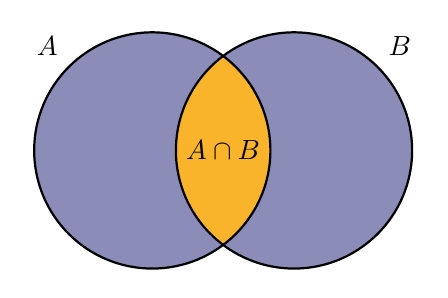
\begin{tikzpicture}[thick,
    set/.style = {circle,
        minimum size = 3cm,
        fill=MidnightBlue!50}]

% Set A
\node[set,label={135:$A$}] (A) at (0,0) {};

% Set B
\node[set,label={45:$B$}] (B) at (1.8,0) {};

% Intersection
\begin{scope}
    \clip (0,0) circle(1.5cm);
    \clip (1.8,0) circle(1.5cm);
    \fill[Dandelion](0,0) circle(1.5cm);
\end{scope}

% Circles outline
\draw (0,0) circle(1.5cm);
\draw (1.8,0) circle(1.5cm);

% Set intersection label
\node at (0.9,0) {$A\cap B$};

\end{tikzpicture}
\end{definicao}

\begin{exemplo}
	Sejam $A = \{1, 2, 3\}$, $B = \{2, 3, 4\}$ e $C = \{r, s, t\}$. Ent\~ao
	\begin{align*}
		A \cap B &= \{2, 3\}\\
		A \cap C &= \emptyset.
	\end{align*}
\end{exemplo}

\begin{definicao}\label{unicao_conjuntos}
	Sejam $A$ e $B$ dois conjuntos. Definimos a \textbf{uni{\~a}o} de $A$ com $B$ como sendo o conjunto $A \cup B$, cujos elementos pertencem ao conjunto $A$ ou ao conjunto $B$. Assim,
	\[
		A \cup B = \{x \mid x \in A \mbox{ ou } x \in B\}.
	\]

    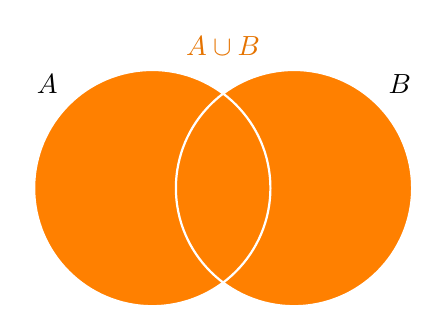
\begin{tikzpicture}[thick,set/.style = {circle,fill=orange,minimum size =3cm}]

        % Set A
        \node [set,label={135:$A$}] (A) at (0,0){};

        % Set B
        \node [set,label={45:$B$}] (B) at (1.8,0){};

        % Circles outline
        \draw[white] (0,0) circle(1.5cm);
        \draw[white] (1.8,0) circle(1.5cm);

        % Union text label
        \node[orange!90!black] at (0.9,1.8) {$A\cup B$};

    \end{tikzpicture}
\end{definicao}

\begin{exemplo}
	Sejam $A = \{1, 2, 3\}$, $B = \{2, 3, 4\}$ e $C = \{r, s, t\}$. Ent\~ao
	\begin{align*}
		A \cup B &= \{1,2,3,4\}\\
		A \cup C &= \{1,2,3,r,s,t\}.
	\end{align*}
\end{exemplo}

\begin{proposicao} Sejam $A$ e $B$ dois conjuntos. Ent{\~a}o:
	\begin{enumerate}[label={\roman*})]
		\item $(A \cap B) \subseteq A$;
		\item $(A \cap B) \subseteq B$;
		\item $A \subseteq A \cup B$;
		\item $B \subseteq A \cup B$.
	\end{enumerate}
\end{proposicao}
\begin{prova}
	Para provar a primeira afirma\c{c}\~ao seja $x \in A \cap B$ um elemento qualquer. Da defini\c{c}\~ao de interse\c{c}\~ao de conjuntos, Defini\c{c}\~ao \ref{intersecao_conjunto}, temos $x \in A$ e $x \in B$. Assim podemos afirmar com certeza que $x \in A$. Logo todo elemente de $A \cap B$ tamb\'em est\'a em $A$, ou seja, $A \cap B \subseteq A$. De modo an\'alogo prova-se a segunda afirma\c{c}\~ao sobre a interse\c{c}\~ao.

	Para a terceira afirma\c{c}\~ao, seja $x \in A$. Da defini\c{c}\~ao de uni\~ao de conjuntos, Defini\c{c}\~ao \ref{unicao_conjuntos}, segue que $x \in A \cup B$. Logo todo elemento de $A$ tamb\'em est\'a em $A \cup B$, ou seja, $A \subseteq (A \cup B)$. De modo an\'alogo prova-se a quarta afirma\c{c}\~ao.
\end{prova}

O conceito de uni{\~a}o ($ \cup $) e intersec{\c c}{\~a}o ($ \cap $) pode ser estendido para mais de dois conjuntos.

\begin{definicao}
	Sejam $A_{1}$, \dots, $A_{n}$ conjuntos. Ent{\~a}o
	\[
		A_{1} \cup A_{2} \cup \cdots \cup A_{n}= \displaystyle\bigcup_{k=1}^n A_{k}
	\]
	{\'e} o conjunto dos elementos $x$ tais que $x$ pertence a pelo menos um dos conjuntos $A_{1}$, \dots, $A_{n}$. Agora,
	\[
		A_{1} \cap \cdots \cap A_{n} = \displaystyle\bigcap_{k=1}^{n}A_{k}
	\]
	{\'e} o conjunto dos elementos $x$ que pertencem a todos os conjuntos $A_{1}$, \dots, $A_{n}$ simultaneamente.
\end{definicao}

\begin{definicao}
	Sejam $A$ e $B$ conjuntos. Se $A \cap B = \emptyset$, dizemos que $A$ e $B$ s{\~a}o \textbf{conjuntos disjuntos}.
\end{definicao}


Sejam $A$ e $B$ conjuntos tais que $C = A \cup B$ e $A \cap B = \emptyset$. Neste caso dizemos que $C$ {\'e} uma \textbf{uni{\~a}o disjunta} de $A$ e $B$. Denotamos tal fato por
\[
	C = A \sqcup B.
\]

\begin{proposicao} Sejam $A,\ B$ e $C$ tr{\^e}s conjuntos, ent{\~a}o:
	\begin{enumerate}[label={\roman*})]
		\item $A \cap (B \cup C) = (A \cap B) \cup (A \cap C)$
		\item $A \cup (B \cap C) = (A \cup B) \cap (A \cup C)$.
	\end{enumerate}
\end{proposicao}
\begin{prova}
	\begin{enumerate}[label={\roman*})]
		\item Precisamos mostrar que
		\begin{enumerate}[label=({\arabic*})]
			\item $A\cap(B\cup C)\subseteq(A\cap B)\cup(A\cap C)$;\label{intersecao_unicao_1}
			\item $(A\cap B)\cup(A\cap C)\subseteq A\cap(B\cup C).$\label{intersecao_unicao_2}
		\end{enumerate}

		Para provar \ref{intersecao_unicao_1} seja $x\in A \cap (B \cup C)$. Logo $x\in A$ e $x\in B\cup C$. Agora, de $x\in B\cup C$, segue que $x\in B$ ou $x\in C$. Suponha que $x\in B$. Como $x\in A$ e $x \in B$, ent\~ao $x\in A\cap B$. Assim, $x\in(A\cap B)\cup(A\cap C)$, ou seja, $A\cap(B\cup C)\subseteq(A\cap B)\cup(A\cap C)$. Por outro lado, se $x\in C$, como $x\in A$, ent{\~a}o $x\in A\cap C$ e da{\'\i} $x\in(A\cap B)\cup(A\cap C)$, logo $A\cap(B\cup C)\subseteq(A\cap B)\cup(A\cap C)$.

		Portanto,
		\[
			A\cap(B\cup C)\subseteq(A\cap B)\cup(A\cap C).
		\]

		Agora para provar \ref{intersecao_unicao_2}, seja $x\in(A\cap B)\cup(A\cap C)$. Da{\'\i}, $x\in A\cap B$ ou $x\in A\cap C$. Suponha que $x\in A\cap B$. Assim, $x\in A$ e $x\in B$. Como $x\in B$, segue que $x\in B\cup C$ e ent{\~a}o $x\in A\cap(B\cup C)$, ou seja, $(A\cap B)\cup(A\cap C)\subseteq A\cap(B\cup C)$. Agora, suponha que $x\in A\cap C$. Com isso $x\in A$ e $x\in C$. Desse modo, $x\in B\cup C$ e ent{\~a}o $x\in A\cap(B\cup C)$ e da{\'\i}
		\[
			(A\cap B)\cup(A\cap C)\subseteq A\cap(B\cup C).
		\]

		Portanto
		\[
			A\cap(B\cup C)=(A\cap B)\cup(A\cap C),
		\]
		como quer{\'\i}amos.
		\item An\'aloga ao caso anterior.
	\end{enumerate}
\end{prova}

\begin{definicao}
	Dados dois conjuntos $A$ e $B$, definimos a \textbf{diferen{\c c}a} dos conjuntos $A$ e $B$, denotada por $A-B$ ou $A\backslash B$ como sendo o conjunto
	\[
		A - B = \{x \mid x \in A \mbox{ e } x \notin B\}.
	\]

    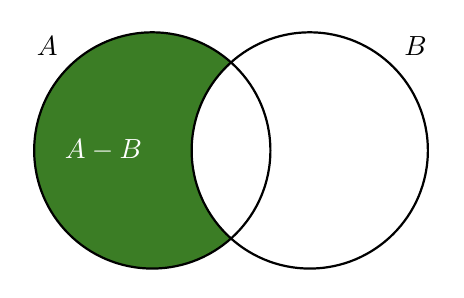
\begin{tikzpicture}[thick,set/.style = { circle, minimum size = 3cm}]

        % Set A
        \node[set,fill=OliveGreen,label={135:$A$}] (A) at (0,0) {};

        % Set B
        \node[set,fill=white,label={45:$B$}] (B) at (0:2) {};

        % Circles outline
        \draw (0,0) circle(1.5cm);
        \draw (2,0) circle(1.5cm);

        % Difference text label
        \node[left,white] at (A.center){$A-B$};

    \end{tikzpicture}
\end{definicao}

\begin{exemplos}
	\begin{enumerate}[label={\arabic*})]
		\item Se $A=\{1,2,3,5,4\}$, $B=\{2,3,6,8\}$, ent\~ao
		\begin{align*}
			A - B &= \{1,4,5\}\\
			B - A &=\{6,8\}.
		\end{align*}
		\item Se $A=\{2,4,6,8,10,...\}$, $B=\{3,6,9,12,15,...\}$, ent\~ao
		\begin{align*}
		 	A - B &= \{2,4,8,10,14,16,...\}\\
		 	B - A &= \{3,9,15,21,...\}
		 \end{align*}
	\end{enumerate}

\end{exemplos}

\begin{proposicao}
	Sejam $A$, $B$ e $C$ conjuntos n\~ao vazios. Ent\~ao
	\[
		(A \cup B) - C = (A - C) \cup (B - C).
	\]
\end{proposicao}
\begin{prova}
	Precisamos mostrar que
	\begin{enumerate}[label={\arabic*})]
		\item $(A \cup B) - C \sub (A - C) \cup (B - C)$
		\item $(B - C) \sub (A \cup B) - C = (A - C)$
	\end{enumerate}
	Para a primeira inclus\~ao seja $x \in (A \cup B) - C$. Assim por defini\c{c}\~ao, $x \in A \cup B$ e $x \notin C$. De $x \in A \cup B$, ent\~ao $x \in A$ ou $x \in B$.

	Se $x \in A$, como $x \notin C$ segue ent\~ao que $x \in A - C$. Logo $x \in (A - C) \cup (B - C)$.

	Se $x \in B$, como $x \notin C$ segue ent\~ao que $x \in B - C$. Logo $x \in (A - C) \cup (B - C)$.

	Assim $(A \cup B) - C = (A - C) \sub (B - C)$.

	Agora, para a segunda inclus\~ao, seja $y \in (A - C) \cup (B - C)$. Por defini\c{c}\~ao, $x \in A - C$ ou $x \in B - C$.

	Se $x \in A - C$, ent\~ao $x \in A$ e $x \notin C$. Como $x \in A$, segue que $x \in A \cup B$. Mas $x \notin C$, com isso, $x \in (A \cup B) - C$.

	Se $x \in B - C$, ent\~ao $x \in B$ e $x \notin C$. Como $x \in B$, segue que $x \in A \cup B$. Mas $x \notin C$, com isso, $x \in (A \cup B) - C$.
	Assim $(A - B) \cup (B - C) \sub (A \cup B) - C$.

	Portanto, $(A \cup B) - C = (A - C) \cup (B - C)$, como quer{\'\i}amos.
\end{prova}

\begin{definicao}
    Dados dois conjuntos $A$ e $E$ tais que $A\subseteq E$, definimos o \textbf{complementar} de $A$ em $E$, denotado $A^C$ ou $C_E(A)$, como
    \[
	    C_E(A) = \{ x \in E \mid x \notin A \}.
    \]

    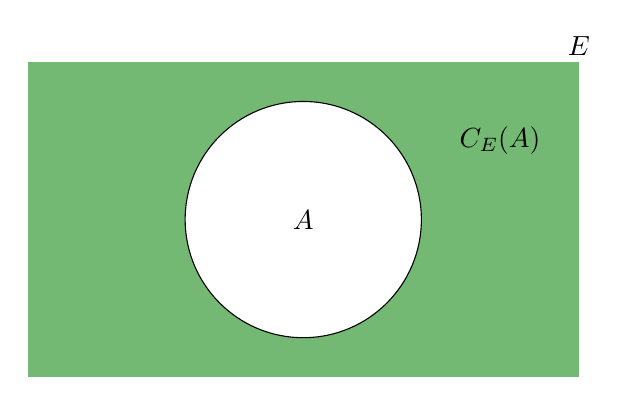
\begin{tikzpicture}
        \fill[Green!55!white, even odd rule](5,-2) rectangle (-2,2) (0:2cm);
        \fill[white] (1.5, 0) circle[radius=1.5];
        \draw[black] (1.5, 0) circle [radius=1.5];

        \node at (1.5, 0) (A) {$A$};
        \node at (4, 1) (C) {$C_E(A)$};
        \node at (5, 2.2) (E) {$E$};
    \end{tikzpicture}
\end{definicao}

\begin{observacoes}
	\begin{enumerate}[label={\arabic*})]
		\item Se $A = E$, ent{\~a}o $C_A(A) = \{ x \in A \mid x \notin A \} = \emptyset$.
		\item $(A^C)^C = \{x \in E \mid x \notin A^C\} = \{ x \in E \mid x \in A \} = A$
	\end{enumerate}

\end{observacoes}

\begin{exemplo}
	Sejam $A = \{1,2,3,4\}$ e $E = \{1,2,3,5,4,0,8,9\}$. Primeiro note que $A \subseteq E$, da{\'\i}
	\[
			A^C = C_E(A) = \{0,5,8,9\}.
	\]
\end{exemplo}

\begin{proposicao}
	Sejam $A$, $B$ e $E$ conjuntos. Se $A\subseteq B\subseteq E$, ent{\~a}o $C_E(B)\subseteq C_E(A)$.
\end{proposicao}
\begin{prova}
	Seja $x \in C_E(B)$. Assim $x\notin B$ e como $A \subseteq B$, ent\~ao $x \notin A$. Da{\'\i} por defini\c{c}\~ao $x\in C_E(A)$, ou seja, $C_E(B) \subseteq C_E(A)$.
\end{prova}

\begin{proposicao} Sejam $A$, $B$ e $E$ tr{\^e}s conjuntos tais que $A\subseteq E$ e $B\subseteq E$. Ent{\~a}o:
\begin{enumerate}[label={\roman*})]
	\item $(A\cup B)^C = A^C\cap B^C$
	\item $(A\cap B)^C = A^C\cup B^C$
\end{enumerate}
\end{proposicao}
\begin{prova}
	\begin{enumerate}[label={\roman*})]
		\item Seja $x \in (A\cup B)^C$. Logo $x\notin A\cup B$, assim $x\notin A$ e $x\notin B$. Da{\'\i}, $x\in A^C$ e $x\in B^C$, isto {\'e}, $x\in A^C\cap B^C$. Desse modo,
		\begin{equation}\label{complementar_uniao-1}
			(A\cup B)^C \subseteq A^C\cap B^C.
		\end{equation}

		Por outro lado, se $x\in A^C\cap B^C$, ent{\~a}o $x\in A^C$ e $x\in B^C$. Com isso, $x\notin A$ e $x\notin B$, ou seja, $x\notin A\cup B$, logo $x\in (A\cup B)^C$. Desse modo
		\begin{equation}\label{complementar_uniao-2}
			A^C\cap B^C\subseteq(A\cup B)^C.
		\end{equation}

		Portanto, de \eqref{complementar_uniao-1} e \eqref{complementar_uniao-2} temos
		\[
			(A\cup B)^C = A^C\cap B^C.
		\]

		\item Seja $x \in (A\cap B)^C$. Logo $x\notin A\cap B$, assim $x\notin A$ ou $x\notin B$. Ent\~ao $x\in A^C$ ou $x\in B^C$, isto {\'e}, $x\in A^C\cup B^C$. Desse modo,
		\begin{equation}\label{complementar_intersecao-1}
			(A\cap B)^C \subseteq A^C\cup B^C.
		\end{equation}

		Por outro lado, se $x\in A^C\cup B^C$, ent{\~a}o $x\in A^C$ ou $x\in B^C$. Da{\'\i}, $x\notin A$ ou $x\notin B$, ou seja, $x\notin A\cap B$, logo $x\in (A\cap B)^C$. Desse modo
		\begin{equation}\label{complementar_intersecao-2}
			A^C\cup B^C\subseteq(A\cap B)^C.
		\end{equation}

		Portanto, de \eqref{complementar_intersecao-1} e \eqref{complementar_intersecao-2} temos
		\[
			(A\cap B)^C = A^C\cup B^C.
		\]
	\end{enumerate}
\end{prova}

\begin{definicao}
	Dados dois conjuntos $A$ e $B$, definimos o \textbf{produto cartesiano} de $A$ por $B$ como sendo o conjunto
	\[
		A \times B = \{(x,y) \mid x\in A, y\in B\}.
	\]
\end{definicao}

Dados $(x,y)$, $(z,t) \in A\times B$, temos
\begin{center}
	$(x,y) = (z,t)$ \textbf{se, e somente se,} $x = z$ \textbf{e} $y = t$.
\end{center}

\begin{exemplo}\label{exemplo_produto_cartesiano}
	Sejam $A = \{1,2\}$ e $B = \{3,4\}$. Ent\~ao
	\begin{align*}
		A \times B &= \{(1,3), (1,4), (2,3), (2,4)\}\\
		B \times A &= \{(3,1), (3,2), (4,1), (4,2)\}
\end{align*}
\end{exemplo}

\begin{observacoes}
	\begin{enumerate}[label={\arabic*})]
		\item Do Exemplo \eqref{exemplo_produto_cartesiano} vemos que em geral $A \times B \neq B\times A$.
		\item No caso em que $A = B$ vamos escrever
		\[
			A \times A = A^2 = \{ (x, y) \mid x, y \in A\}.
		\]
		De modo geral:
		\[
			\underbrace{A \times A \times \cdots \times A}_{n\ vezes} = A^n = \{ (x_1, x_2, \dots, x_n) \mid x_1, x_2, \dots, x_n \in A\}
		\]
		para $n \ge 2$.
	\end{enumerate}
\end{observacoes}

\begin{definicao}
	Para qualquer conjunto $A$, indicamos por $\mathcal{P}(A)$ o conjunto
	\[
		\mathcal{P}(A) = \{ X \mid X\subseteq A\}
	\]
	que \'e chamado de \textbf{conjunto das partes} de $A$.
\end{definicao}

Os elementos desse conjunto s{\~a}o todos os subconjuntos de $A$. Dizer que $Y\in \mathcal{P}(A)$ significa que $Y \subseteq A$. Particularmente, temos $\emptyset\in \mathcal{P}(A)$ e $A\in \mathcal{P}(A)$.

\begin{exemplos}
	\begin{enumerate}[label={\arabic*})]
		\item $A = \emptyset$, $\mathcal{P}(A) = \{\emptyset\}$;
		\item $B = \{x\}$, $\mathcal{P}(B) = \{\emptyset, \{x\}\}$;
		\item $C = \{a,b,c\}$, $\mathcal{P}(C)=\{\emptyset, \{a\}, \{b\},\{c\},\{a,b\},\{a,c\},\{b,c\},C\}$;
		\item $D=\real$, $\mathcal{P}(D)=\{X\mid X \subseteq \real\}$, por exemplo $\rac\in \mathcal{P}(D)$.
	\end{enumerate}
\end{exemplos}
